%!TEX root = physical_authent.tex
\subsubsection{Experimental Setup.}
In our experiments, we considered a verifier that executes an AES-$128$ (\emph{i.e.} $N_r= 10$) and targets only two internal states per AES round, namely the states after applying the AddRoundKey and SubBytes (these states are denoted by $X$ and $Y$ in Algorithm~\ref{alg:AES}). 
Moreover, two different scenarios are studied. In the first one, the verifier focuses on the first round of each AES execution yielding $32$ sensitive variables. In the second scenario, the verifier considers three rounds per AES execution yielding $32\times 3 = 96$ targeted variables. The corresponding physical leakage was acquired using the ChipWhisperer-Lite board~\cite{ChipWhisperer}. Furthermore, for robust statistics we instantiated $q = 1000$.
\add{The choice of the ChipWhisperer acquisition board is motivated by its simplicity and that the corresponding leakage model fits well our assumption in~\eqref{eq:leak}. Indeed, our protocol is intended for contactless device which implies that the corresponding leakage should be more noisy compared to the ChipWhisperer one. In the sequel, we consider this scenario by performing our experiments in a very noisy environment.}

\subsubsection{Assessment of our Proposal in a (almost) Noise-Free Environment.}
In the following, we considered a genuine prover (\emph{i.e.} the acquired leakage corresponds to $N$ AES executions using the correct session keys derived from the master key $K$).
Then, for each scenario, we plotted the correct likelihood value $\mathcal{L}_0$ (the red curve) and the estimated mean $\mu_{\not={0}}$ and mean deviation $w_{\not={0}}$ of the random variable \(\Lambda_{\not={0}}\) (the blue dotted curve and bars) according to an increasing number $N$ of AES executions.
The obtained results in both scenarios are illustrated in Fig.~\ref{fig:likely_grow}.

From Fig.~\ref{fig:likely_grow}, it is obvious that increasing the number $N$ of executed AES enlarges the gap between $\mathcal{L}_0$ and $\{\mathcal{L}_{i \ne 0}\}$ when the prover is genuine. Moreover, one can conclude that the verifier is able to identify a genuine prover within merely $N=10$ AES executions. Furthermore, considering more  sensitive variables as shown in Fig.~\ref{sfig:threeRounds_incN}, the gap between $\mathcal{L}_0$ and $\{\mathcal{L}_{i \ne 0}\}$ increases while the deviation margin decreases.

\begin{figure}[ht!]
      \subfloat[][One round]{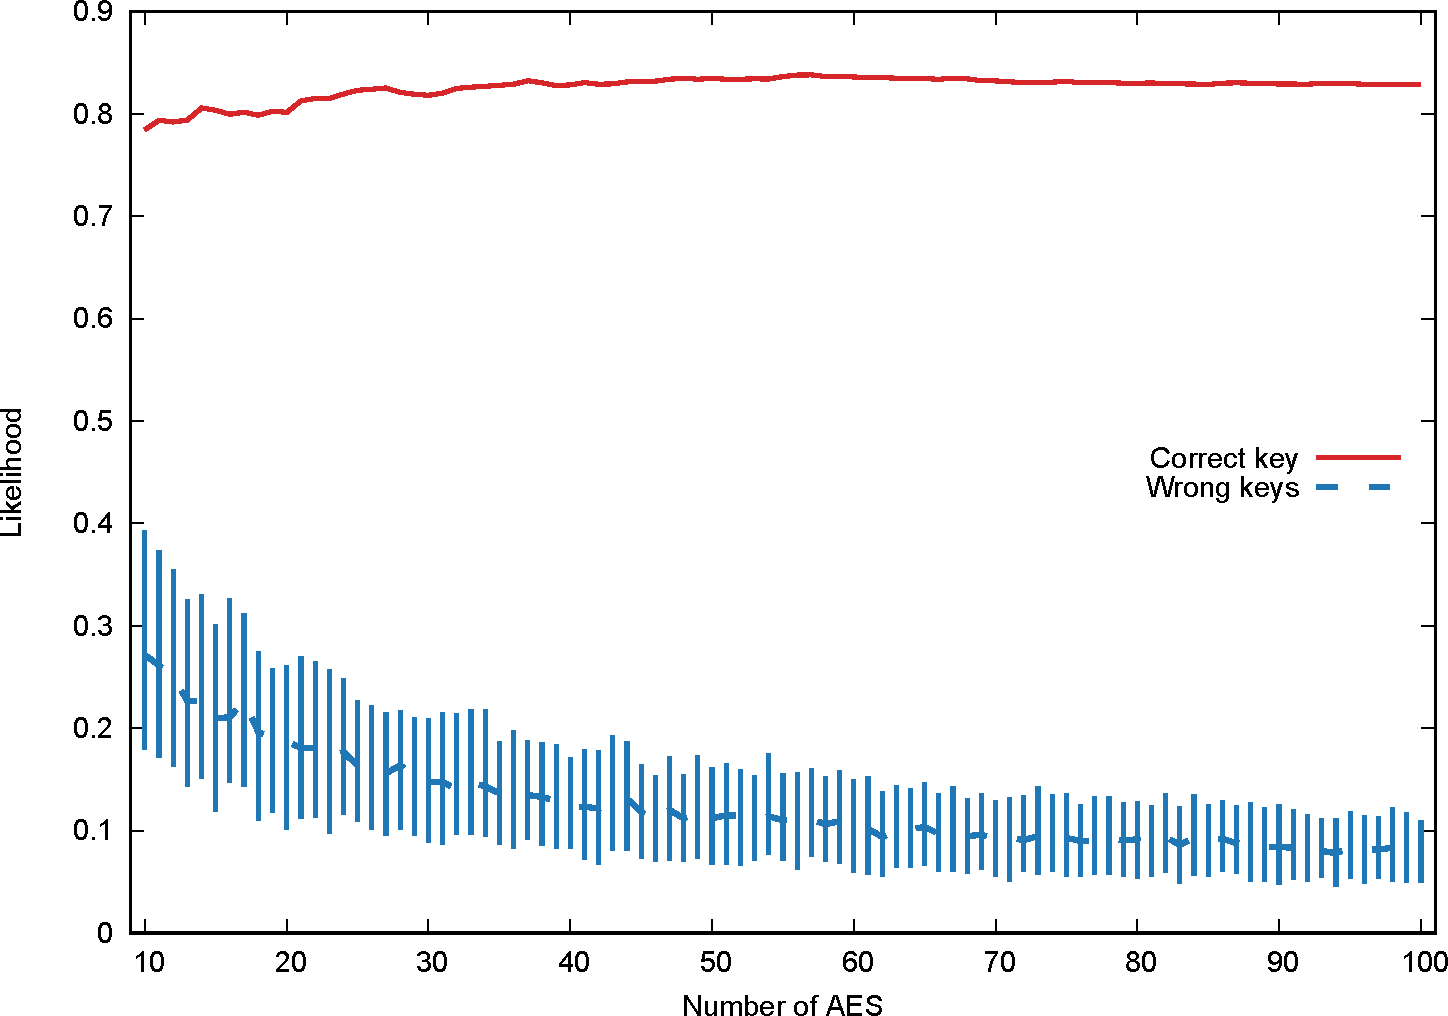
\includegraphics[width=0.5\linewidth]
      {prog_cpa_1r}\label{sfig:oneRound_incN}}
      \subfloat[][Three rounds]{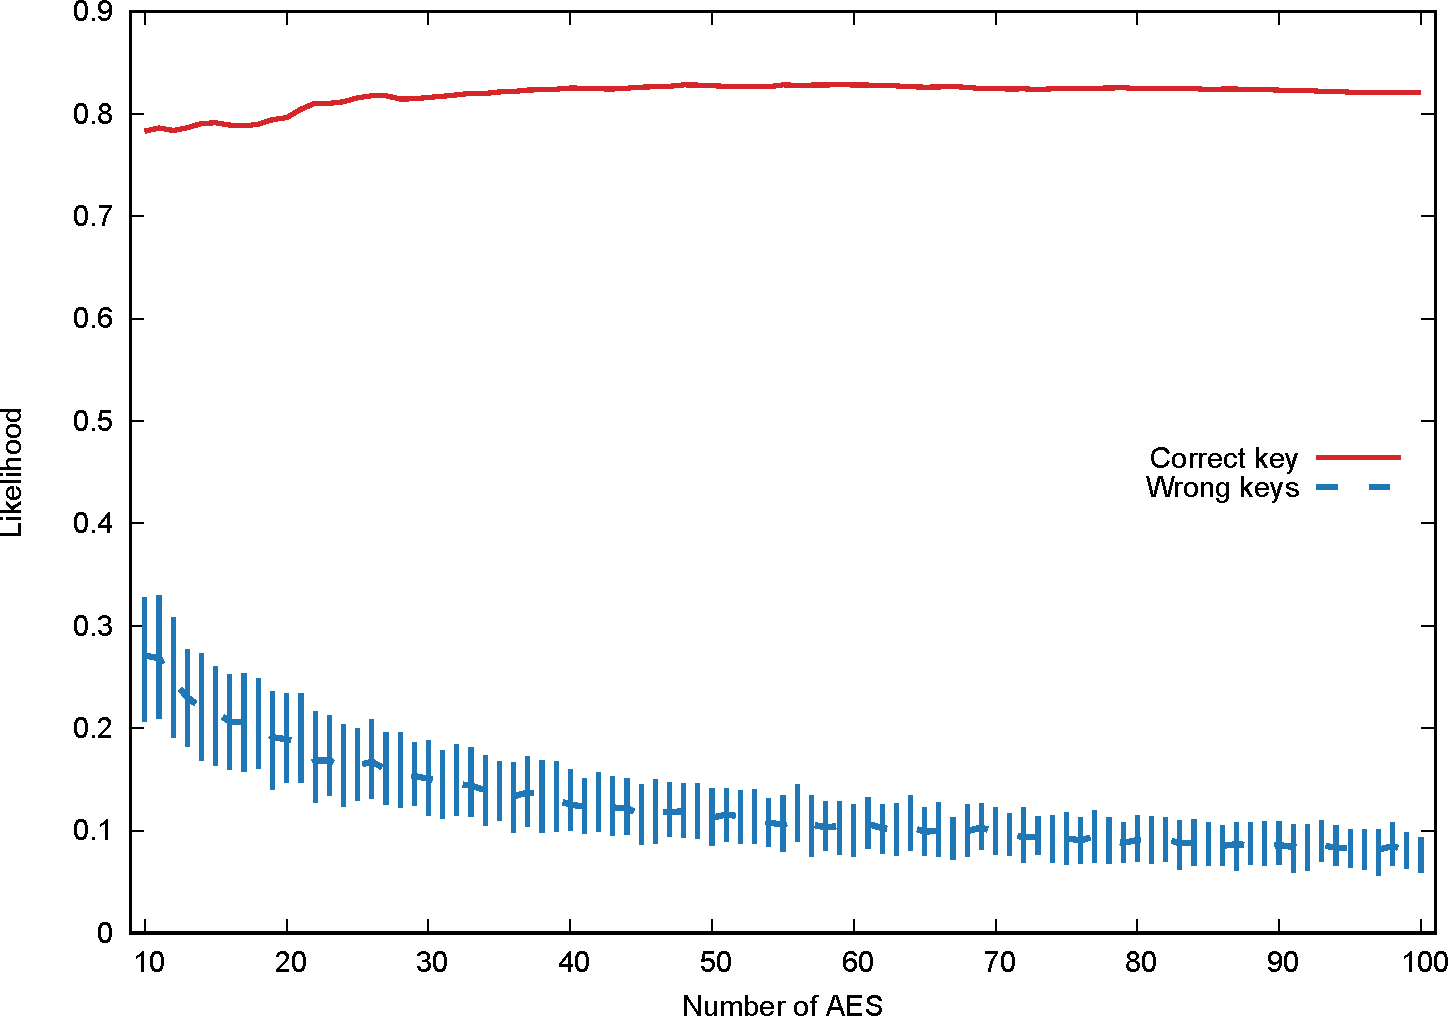
\includegraphics[width=0.5\linewidth]
      {prog_cpa_3r}\label{sfig:threeRounds_incN}}
\caption{Evolution of the likelihood according to an increasing number of AES executions.}\label{fig:likely_grow}
\end{figure}

\subsubsection{Assessment of our Proposal in a Noisy Environment.}
It is well-known that the ChipWhisperer-Lite is mostly noise-free\footnote{According to our measurements, it follows a Gaussian distribution with a standard deviation of $\approx 0.004$.}. To demonstrate the efficiency of our proposal in a noisy environment, the same acquired trace was reused to artificially increase the noise level (\emph{i.e.} by adding a white Gaussian noise).
We plotted in Fig.~\ref{fig:FRRwh} the evolution of the acceptance rate according to an increasing noise standard deviation and a fixed number of executed AES ($N=20$).

As expected, the acceptance rate decreases when the noise standard deviation increases. Moreover, for a fixed noise standard deviation, the more internal states, the higher the acceptance rate.
Finally, we repeated the same experiments when increasing the number of executed AES and  used the Signal-to-Noise Ratio (SNR) rather than the noise standard deviation to better quantify the amount of white noise which is added. The obtained results are depicted in Fig.~\ref{fig:fixed_noised}.

\begin{figure}[ht!]
\centering
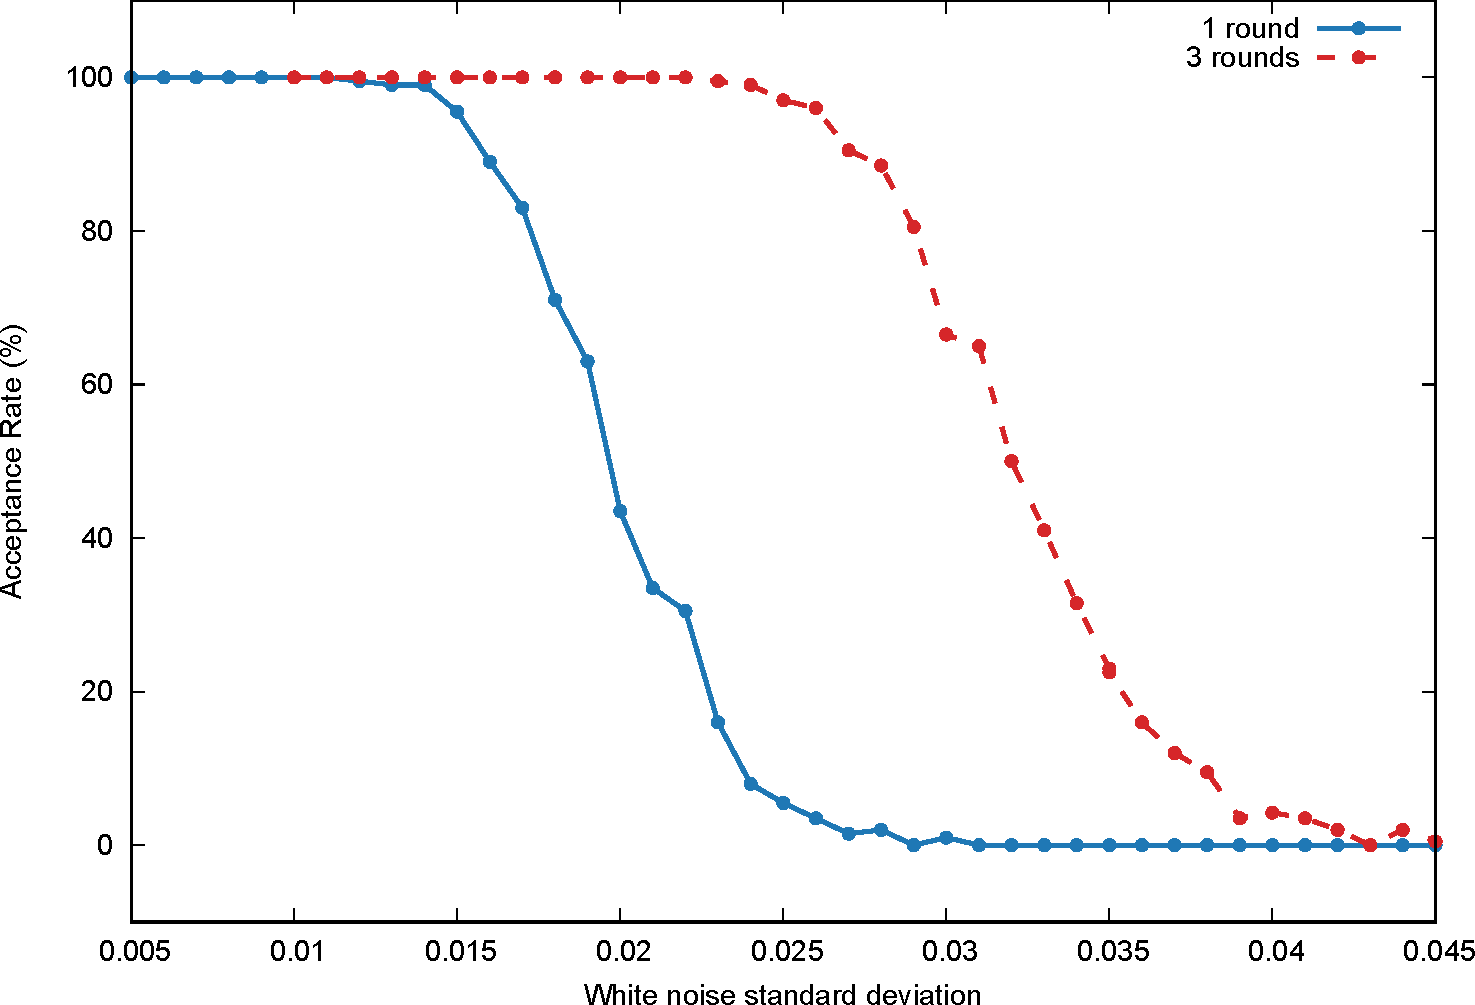
\includegraphics[width=0.9\linewidth]{prob.pdf}
\caption{Evolution of the acceptance rate according to an increasing noise standard deviation and a fixed number of executed AES.}\label{fig:FRRwh}
\end{figure}

\begin{figure}[ht!]
\centering
      \subfloat[][One round]{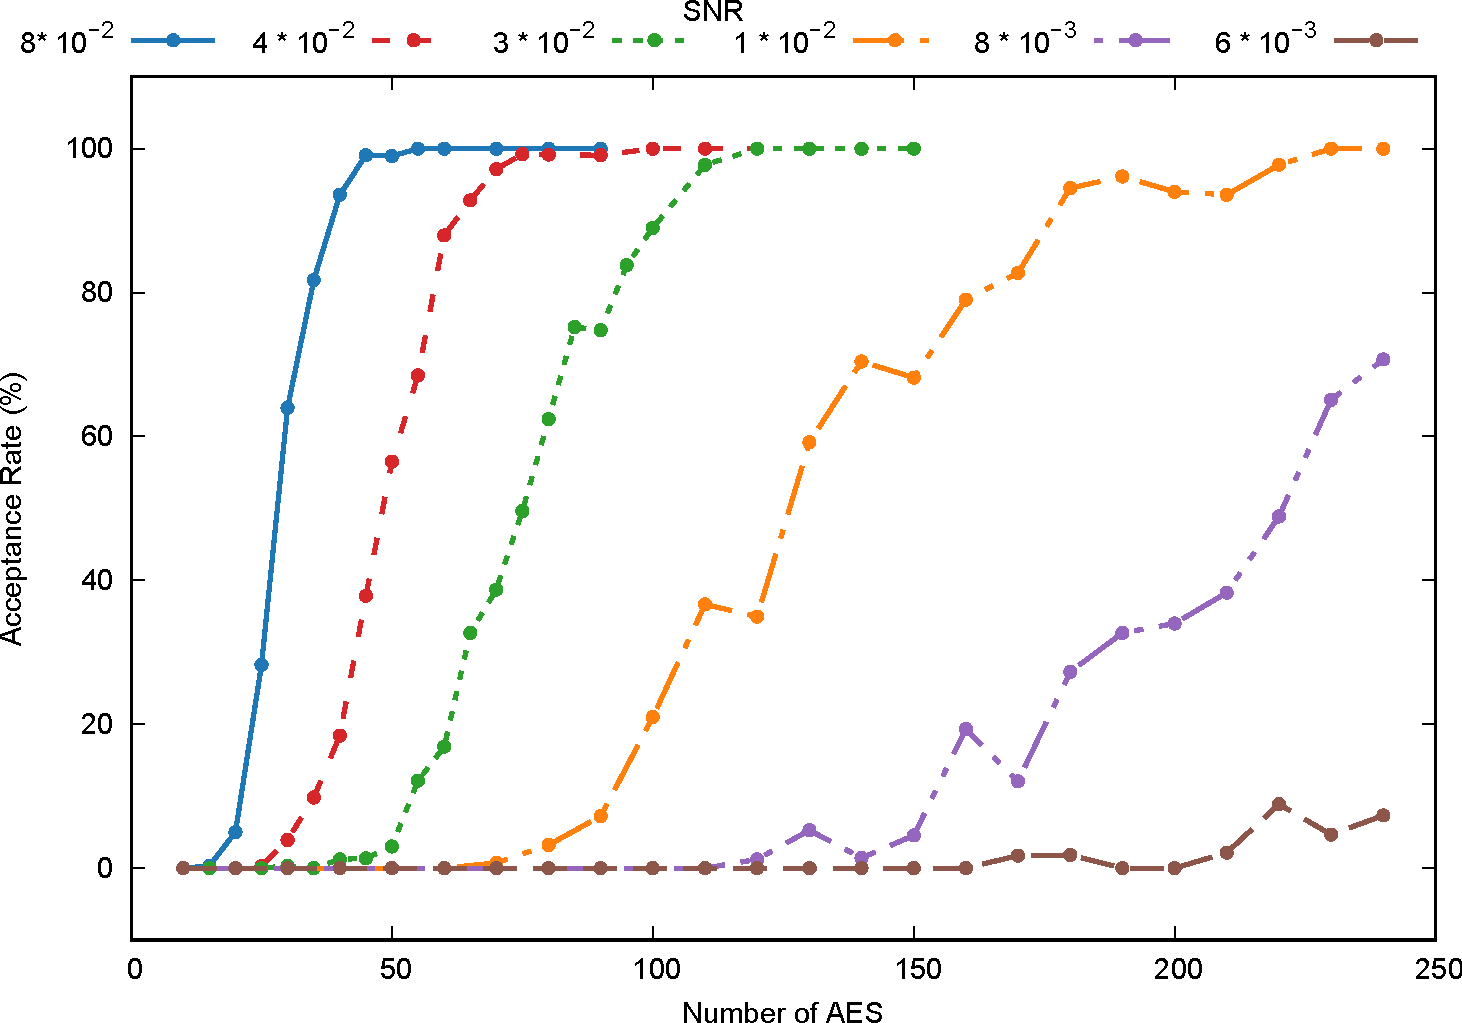
\includegraphics[width=0.5\linewidth]
      {noise_prob_cpa.pdf}\label{sfig:oneRound_incNoise}}
      \subfloat[][Three rounds]{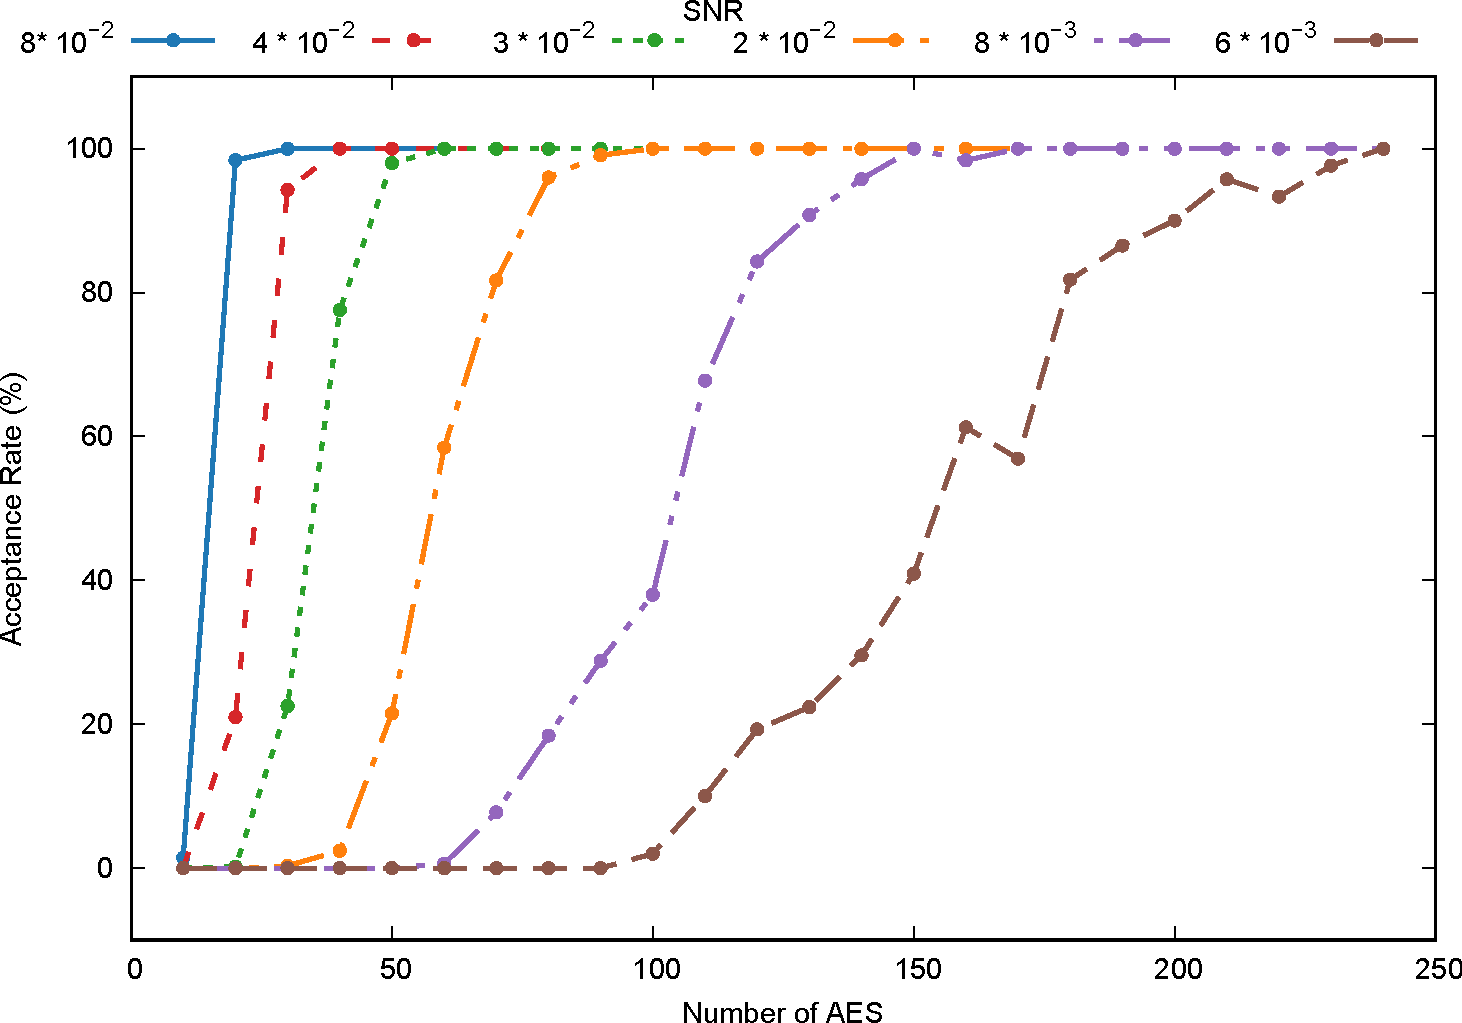
\includegraphics[width=0.5\linewidth]
      {noise_prob_cpa_3r.pdf}\label{sfig:threeRounds_incNoise}}   
\caption{Evolution of the acceptance rate according to an increasing number of executed AES and SNR.}\label{fig:fixed_noised}
\end{figure}
	
From Fig.~\ref{fig:fixed_noised}, one can conclude that in the presence of a significant amount of noise, increasing the number $N$ of AES executions allows the verifier to better distinguish the presence of a genuine prover. Moreover, the number of variables used for the likelihood computation is also of great interest. Indeed, by considering more AES rounds and more internal states per round, the verifier increases the acceptance rate while executing less AES computations.

\add{Regarding the choice of the optimal parameters (\emph{i.e.} number of AES, number of rounds, \dots), it is up to the designer to choose the suitable ones with respect to the the noise level and the required acceptance rate.}


\subsubsection{FAR and FRR Assessment.}\label{ssec:FARFRR}
In this section, we evaluated our proposed authentication protocol with respect to two well-known security metrics: the  \textit{False Acceptance Rate} (FAR) and the \textit{False Rejection Rate} (FRR).
The FAR is the measure of probability that an authentication protocol accepts an unauthorized prover while the FRR is the measure of probability that an authentication protocol rejects a genuine prover.

To do so, we considered in the following an authentication between a verifier and a malicious prover.
We acquired one trace on the ChipWhisperer board corresponding to $N$ executions of leaky AES using wrong session keys at the prover side. We stress the fact that the noise level is similar to the experiments reported in Fig.\ref{sfig:threeRounds_incN} (\emph{i.e.} $\sigma \approx 0.004$). Then, we plotted in Fig.~\ref{fig:proxTest} the evolution of the likelihood $\mathcal{L}_0$ (the red curve) and the estimated mean and mean deviation $(\mu_{\not={0}}, w_{\not={0}})$ of $\Lambda_{\not={0}}$ (the blue dotted curve and bars) according to an increasing number of executed AES when considering three rounds per AES execution.

\begin{figure}[ht!]
\centering
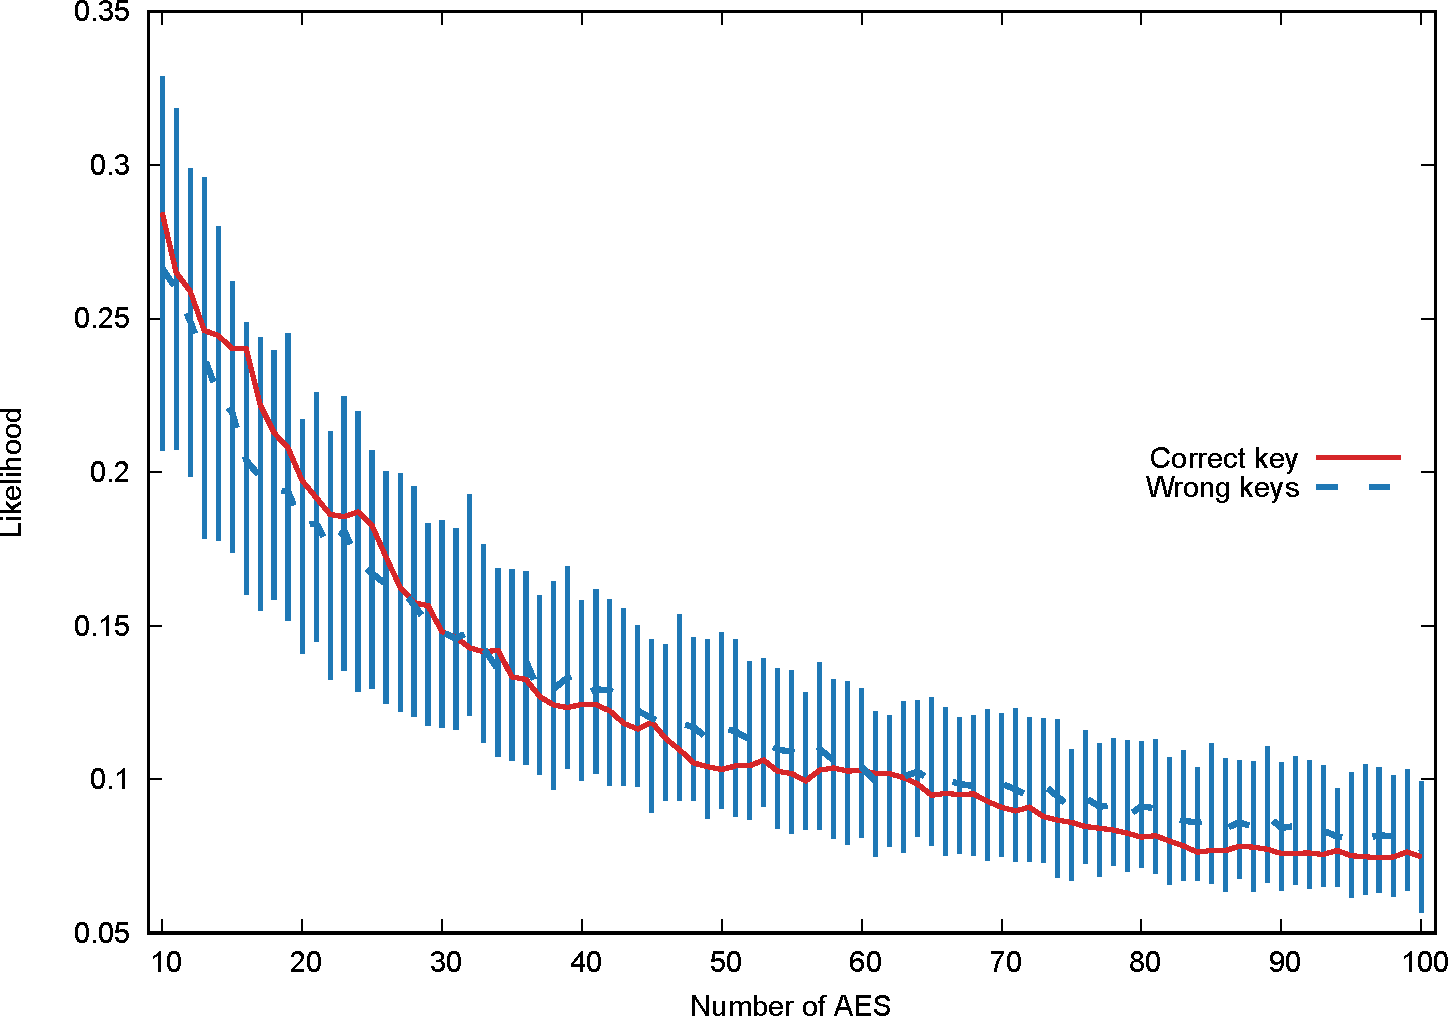
\includegraphics[width=0.7\linewidth]{prog_cpa_3r_false.pdf}
\caption{Evolution of the likelihood according to an increasing number of AES executions when considering a malicious prover.}
\label{fig:proxTest}
\end{figure}

From Fig.~\ref{fig:proxTest}, one can see that the curves overlap and hence the verifier concludes that the prover is a malicious one and rejects the authentication.
So, the obtained results confirm that the FAR of our proposed authentication protocol is almost zero independently of the number of executed AES. We recall that, by design, the theoretical FAR is $2^{-128}$ which the probability that a malicious prover guesses correctly the $128$-bit shared master key $K$. 

Regarding the FRR, we demonstrated in Fig.~\ref{fig:fixed_noised} that in the presence of a genuine prover the acceptance rate decreases (\emph{i.e.} the FRR increases) when the noise standard deviation increases. On the other hand, when the number of executed AES increases and/or when considering several intermediate values then the acceptance rate increases too. This implies that, depending on the application, one can adjust the FRR by tuning the number of executed AES and the number of targeted intermediate values with respect to the noise level. This can be done as a beforehand agreement between the genuine prover and the verifier.